\documentclass{article}
\usepackage[utf8]{inputenc}
\usepackage[cm]{fullpage}
\usepackage{amssymb}
\usepackage{multicol}
\usepackage{graphicx}
\usepackage{multicol}

\renewcommand{\emph}[1]{\textbf{#1}}

%\newcommand{\mycell}[3]{ #1 & #2 & \parbox{12cm}{#3} \\ \hline }
\newcommand{\mycell}[3]{

  #1 & #2 & \parbox{6cm}{
    \vspace{.1\baselineskip}
    #3
    \vspace{.1\baselineskip}
  } \\ \hline
}
\newcommand{\titulo}[1]{{\bf #1}}

\newcommand{\itspc}{
  \vspace{-8pt}
  \setlength\itemsep{-2pt}
}

\begin{document}

\pagenumbering{gobble}

\begin{center}
{\Large \bf Primeiro Trabalho de Elementos de Lógica Digital - 2015/2}
\\
10/09/2015
\vspace{5mm}
\end{center}

\noindent
\titulo{Professor:} Marcos Daniel Baroni $<$\texttt{marcos.baroni@aluno.ufes.br}$>$

\noindent
\titulo{Data de entrega:} 1º de outubro de 2015

\noindent
\titulo{Regras:}
\begin{enumerate}
  \itspc
  \item O trabalho será feito em dupla;
  \item \underline{Não será tolerado plágio.} Trabalhos copiados serão penalizados com nota zero.
\end{enumerate}

\noindent
\titulo{Ferramenta para simulação:} Logisim (\texttt{http://www.cburch.com/logisim/})

\noindent
\titulo{Material a ser entregue:}
\begin{enumerate}
  \itspc
  \item{Arquivo de simulação}:
  \begin{itemize}
    \itspc
    \item{Enviar por email para \texttt{marcos.baroni@aluno.ufes.br} com arquivo em anexo;}
    \item{O título do email deve estar no formato \texttt{"ELD:TRAB1:$<$mbaroni$><$jsilva$>$"};}
    \item{Apenas um arquivo (\texttt{.circ}) será entregue, contendo os circuitos simulados.}
  \end{itemize}
  \item{Resolução (em papel):
  \begin{itemize}
    \itspc
    \item{Entregar em mãos no dia 1º/10 as resoluções das simulações;}
    \item{Podem estar manuscritas, desde que estejam claras e organizadas.
\underline{A clareza e a organização serão avaliadas};}
    \item{As resoluções devem conter breves explicações por extenso dos passos realizados.}
  \end{itemize}
}
\end{enumerate}

\noindent
\titulo{\large Simulação 1} \\
Projetar e implementar um circuito para controle de um display de 7 segmentos capaz de escreve os digitos de $0$ a $9$ tendo como entrada os dígitos em código Gray.
\\

\begin{center}
%\begin{multicols}{2}
%\begin{tabular}{|c|c|}
%  \hline
%  {\bf Dec.} & {\bf Gray} \\ \hline
%  0 & 0000 \\
%  1 & 0001 \\
%  2 & 0011 \\
%  3 & 0010 \\
%  4 & 0110 \\
%  5 & 0111 \\
%  6 & 0101 \\
%  7 & 0100 \\
%  8 & 1100 \\
%  9 & 1101 \\
%  \hline
%\end{tabular}
%\\
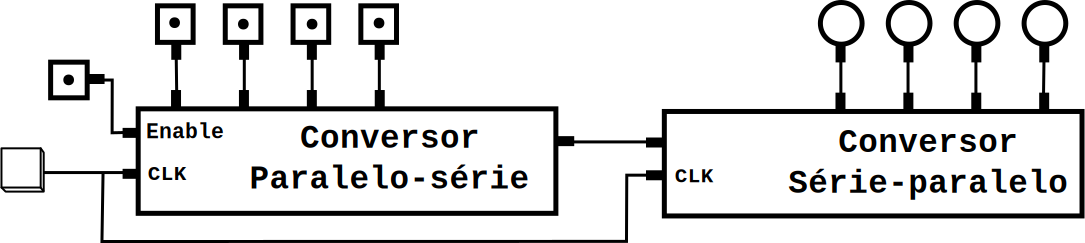
\includegraphics[scale=0.3]{sim1}
%\end{multicols}
\end{center}

\vspace{3mm}
\noindent
\titulo{\large Simulação 2} \\
Projetar e implementar um circuito decodificador de código BCD8421 para código Gray.
Utilizá-lo acoplado ao circuito de controle projetado na Simulação 1 para controlar o display de 7 segmentos.
\\
\begin{center}
%\begin{multicols}{2}
%\begin{tabular}{|c|c|c|}
%  \hline
%  {\bf Dec.} & {\bf BCD8421} & {\bf Gray} \\ \hline
%  0 & 0000 & 0000 \\
%  1 & 0001 & 0001 \\
%  2 & 0010 & 0011 \\
%  3 & 0011 & 0010 \\
%  4 & 0100 & 0110 \\
%  5 & 0101 & 0111 \\
%  6 & 0110 & 0101 \\
%  7 & 0111 & 0100 \\
%  8 & 1000 & 1100 \\
%  9 & 1001 & 1101 \\
%  \hline
%\end{tabular}
%\\
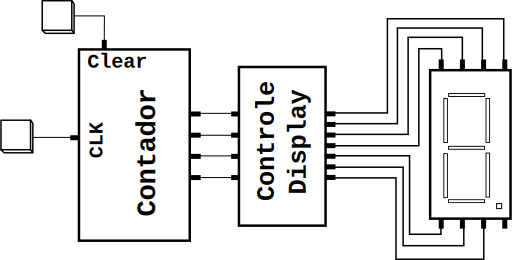
\includegraphics[scale=0.3]{sim2}
%\end{multicols}
\end{center}

\end{document}

